% Created by tikzDevice version 0.12.6 on 2024-02-18 17:32:40
% !TEX encoding = UTF-8 Unicode
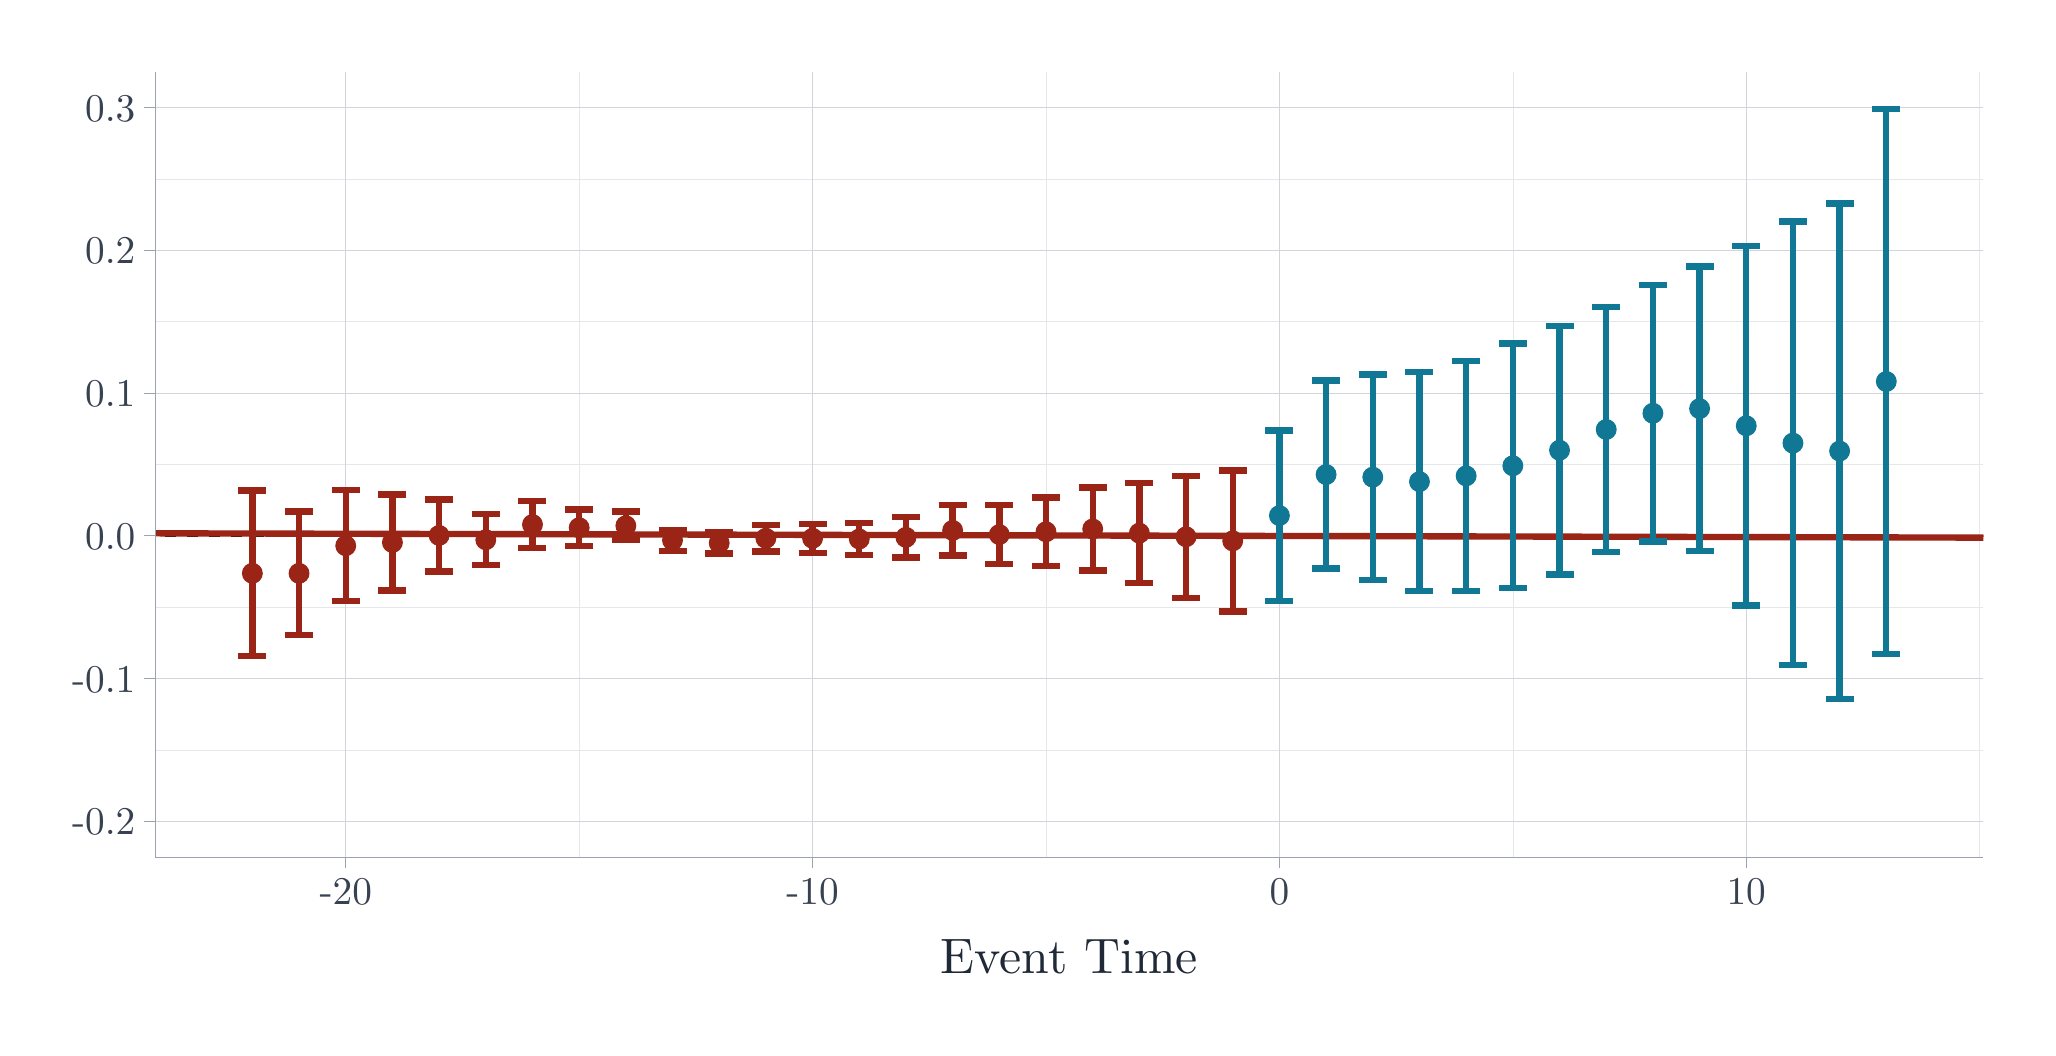
\begin{tikzpicture}[x=1pt,y=1pt]
\definecolor{fillColor}{RGB}{255,255,255}
\path[use as bounding box,fill=fillColor] (0,0) rectangle (722.70,361.35);
\begin{scope}
\path[clip] (  0.00,  0.00) rectangle (722.70,361.35);
\definecolor{drawColor}{RGB}{255,255,255}

\path[draw=drawColor,line width= 0.8pt,line join=round,line cap=round,fill=fillColor] (  0.00,  0.00) rectangle (722.70,361.35);
\end{scope}
\begin{scope}
\path[clip] ( 46.10, 61.65) rectangle (706.70,345.35);
\definecolor{drawColor}{RGB}{255,255,255}
\definecolor{fillColor}{RGB}{255,255,255}

\path[draw=drawColor,line width= 0.8pt,line join=round,line cap=round,fill=fillColor] ( 46.10, 61.65) rectangle (706.70,345.35);
\definecolor{drawColor}{RGB}{229,231,235}

\path[draw=drawColor,line width= 0.2pt,line join=round] ( 46.10,100.34) --
	(706.70,100.34);

\path[draw=drawColor,line width= 0.2pt,line join=round] ( 46.10,151.92) --
	(706.70,151.92);

\path[draw=drawColor,line width= 0.2pt,line join=round] ( 46.10,203.50) --
	(706.70,203.50);

\path[draw=drawColor,line width= 0.2pt,line join=round] ( 46.10,255.08) --
	(706.70,255.08);

\path[draw=drawColor,line width= 0.2pt,line join=round] ( 46.10,306.66) --
	(706.70,306.66);

\path[draw=drawColor,line width= 0.2pt,line join=round] (199.28, 61.65) --
	(199.28,345.35);

\path[draw=drawColor,line width= 0.2pt,line join=round] (367.97, 61.65) --
	(367.97,345.35);

\path[draw=drawColor,line width= 0.2pt,line join=round] (536.66, 61.65) --
	(536.66,345.35);

\path[draw=drawColor,line width= 0.2pt,line join=round] (705.35, 61.65) --
	(705.35,345.35);
\definecolor{drawColor}{RGB}{209,213,219}

\path[draw=drawColor,line width= 0.4pt,line join=round] ( 46.10, 74.55) --
	(706.70, 74.55);

\path[draw=drawColor,line width= 0.4pt,line join=round] ( 46.10,126.13) --
	(706.70,126.13);

\path[draw=drawColor,line width= 0.4pt,line join=round] ( 46.10,177.71) --
	(706.70,177.71);

\path[draw=drawColor,line width= 0.4pt,line join=round] ( 46.10,229.29) --
	(706.70,229.29);

\path[draw=drawColor,line width= 0.4pt,line join=round] ( 46.10,280.87) --
	(706.70,280.87);

\path[draw=drawColor,line width= 0.4pt,line join=round] ( 46.10,332.45) --
	(706.70,332.45);

\path[draw=drawColor,line width= 0.4pt,line join=round] (114.93, 61.65) --
	(114.93,345.35);

\path[draw=drawColor,line width= 0.4pt,line join=round] (283.62, 61.65) --
	(283.62,345.35);

\path[draw=drawColor,line width= 0.4pt,line join=round] (452.31, 61.65) --
	(452.31,345.35);

\path[draw=drawColor,line width= 0.4pt,line join=round] (621.00, 61.65) --
	(621.00,345.35);
\definecolor{drawColor}{RGB}{0,0,0}

\path[draw=drawColor,line width= 0.9pt,dash pattern=on 4pt off 4pt ,line join=round] (-614.49,177.71) -- (1367.30,177.71);
\definecolor{drawColor}{RGB}{154,36,21}

\path[draw=drawColor,line width= 2.3pt,line join=round] (-614.49,180.20) -- (1367.30,175.51);
\definecolor{fillColor}{RGB}{154,36,21}

\path[draw=drawColor,line width= 0.4pt,line join=round,line cap=round,fill=fillColor] ( 81.19,164.18) circle (  3.57);

\path[draw=drawColor,line width= 0.4pt,line join=round,line cap=round,fill=fillColor] ( 98.06,164.18) circle (  3.57);

\path[draw=drawColor,line width= 0.4pt,line join=round,line cap=round,fill=fillColor] (114.93,174.15) circle (  3.57);

\path[draw=drawColor,line width= 0.4pt,line join=round,line cap=round,fill=fillColor] (131.80,175.32) circle (  3.57);

\path[draw=drawColor,line width= 0.4pt,line join=round,line cap=round,fill=fillColor] (148.67,177.87) circle (  3.57);

\path[draw=drawColor,line width= 0.4pt,line join=round,line cap=round,fill=fillColor] (165.54,176.30) circle (  3.57);

\path[draw=drawColor,line width= 0.4pt,line join=round,line cap=round,fill=fillColor] (182.41,181.80) circle (  3.57);

\path[draw=drawColor,line width= 0.4pt,line join=round,line cap=round,fill=fillColor] (199.28,180.64) circle (  3.57);

\path[draw=drawColor,line width= 0.4pt,line join=round,line cap=round,fill=fillColor] (216.15,181.36) circle (  3.57);

\path[draw=drawColor,line width= 0.4pt,line join=round,line cap=round,fill=fillColor] (233.01,176.14) circle (  3.57);

\path[draw=drawColor,line width= 0.4pt,line join=round,line cap=round,fill=fillColor] (249.88,175.13) circle (  3.57);

\path[draw=drawColor,line width= 0.4pt,line join=round,line cap=round,fill=fillColor] (266.75,176.85) circle (  3.57);

\path[draw=drawColor,line width= 0.4pt,line join=round,line cap=round,fill=fillColor] (283.62,176.84) circle (  3.57);

\path[draw=drawColor,line width= 0.4pt,line join=round,line cap=round,fill=fillColor] (300.49,176.58) circle (  3.57);

\path[draw=drawColor,line width= 0.4pt,line join=round,line cap=round,fill=fillColor] (317.36,177.18) circle (  3.57);

\path[draw=drawColor,line width= 0.4pt,line join=round,line cap=round,fill=fillColor] (334.23,179.68) circle (  3.57);

\path[draw=drawColor,line width= 0.4pt,line join=round,line cap=round,fill=fillColor] (351.10,178.18) circle (  3.57);

\path[draw=drawColor,line width= 0.4pt,line join=round,line cap=round,fill=fillColor] (367.97,179.19) circle (  3.57);

\path[draw=drawColor,line width= 0.4pt,line join=round,line cap=round,fill=fillColor] (384.84,180.19) circle (  3.57);

\path[draw=drawColor,line width= 0.4pt,line join=round,line cap=round,fill=fillColor] (401.71,178.70) circle (  3.57);

\path[draw=drawColor,line width= 0.4pt,line join=round,line cap=round,fill=fillColor] (418.58,177.38) circle (  3.57);

\path[draw=drawColor,line width= 0.4pt,line join=round,line cap=round,fill=fillColor] (435.44,175.90) circle (  3.57);
\definecolor{drawColor}{RGB}{16,120,149}
\definecolor{fillColor}{RGB}{16,120,149}

\path[draw=drawColor,line width= 0.4pt,line join=round,line cap=round,fill=fillColor] (452.31,185.05) circle (  3.57);

\path[draw=drawColor,line width= 0.4pt,line join=round,line cap=round,fill=fillColor] (469.18,199.87) circle (  3.57);

\path[draw=drawColor,line width= 0.4pt,line join=round,line cap=round,fill=fillColor] (486.05,198.93) circle (  3.57);

\path[draw=drawColor,line width= 0.4pt,line join=round,line cap=round,fill=fillColor] (502.92,197.31) circle (  3.57);

\path[draw=drawColor,line width= 0.4pt,line join=round,line cap=round,fill=fillColor] (519.79,199.39) circle (  3.57);

\path[draw=drawColor,line width= 0.4pt,line join=round,line cap=round,fill=fillColor] (536.66,203.03) circle (  3.57);

\path[draw=drawColor,line width= 0.4pt,line join=round,line cap=round,fill=fillColor] (553.53,208.66) circle (  3.57);

\path[draw=drawColor,line width= 0.4pt,line join=round,line cap=round,fill=fillColor] (570.40,216.15) circle (  3.57);

\path[draw=drawColor,line width= 0.4pt,line join=round,line cap=round,fill=fillColor] (587.27,222.02) circle (  3.57);

\path[draw=drawColor,line width= 0.4pt,line join=round,line cap=round,fill=fillColor] (604.14,223.69) circle (  3.57);

\path[draw=drawColor,line width= 0.4pt,line join=round,line cap=round,fill=fillColor] (621.00,217.48) circle (  3.57);

\path[draw=drawColor,line width= 0.4pt,line join=round,line cap=round,fill=fillColor] (637.87,211.23) circle (  3.57);

\path[draw=drawColor,line width= 0.4pt,line join=round,line cap=round,fill=fillColor] (654.74,208.36) circle (  3.57);

\path[draw=drawColor,line width= 0.4pt,line join=round,line cap=round,fill=fillColor] (671.61,233.50) circle (  3.57);
\definecolor{drawColor}{RGB}{154,36,21}

\path[draw=drawColor,line width= 2.3pt,line join=round] ( 76.13,194.08) --
	( 86.25,194.08);

\path[draw=drawColor,line width= 2.3pt,line join=round] ( 81.19,194.08) --
	( 81.19,134.27);

\path[draw=drawColor,line width= 2.3pt,line join=round] ( 76.13,134.27) --
	( 86.25,134.27);

\path[draw=drawColor,line width= 2.3pt,line join=round] ( 93.00,186.49) --
	(103.12,186.49);

\path[draw=drawColor,line width= 2.3pt,line join=round] ( 98.06,186.49) --
	( 98.06,141.88);

\path[draw=drawColor,line width= 2.3pt,line join=round] ( 93.00,141.88) --
	(103.12,141.88);

\path[draw=drawColor,line width= 2.3pt,line join=round] (109.87,194.23) --
	(119.99,194.23);

\path[draw=drawColor,line width= 2.3pt,line join=round] (114.93,194.23) --
	(114.93,154.08);

\path[draw=drawColor,line width= 2.3pt,line join=round] (109.87,154.08) --
	(119.99,154.08);

\path[draw=drawColor,line width= 2.3pt,line join=round] (126.74,192.70) --
	(136.86,192.70);

\path[draw=drawColor,line width= 2.3pt,line join=round] (131.80,192.70) --
	(131.80,157.93);

\path[draw=drawColor,line width= 2.3pt,line join=round] (126.74,157.93) --
	(136.86,157.93);

\path[draw=drawColor,line width= 2.3pt,line join=round] (143.61,190.86) --
	(153.73,190.86);

\path[draw=drawColor,line width= 2.3pt,line join=round] (148.67,190.86) --
	(148.67,164.88);

\path[draw=drawColor,line width= 2.3pt,line join=round] (143.61,164.88) --
	(153.73,164.88);

\path[draw=drawColor,line width= 2.3pt,line join=round] (160.48,185.50) --
	(170.60,185.50);

\path[draw=drawColor,line width= 2.3pt,line join=round] (165.54,185.50) --
	(165.54,167.11);

\path[draw=drawColor,line width= 2.3pt,line join=round] (160.48,167.11) --
	(170.60,167.11);

\path[draw=drawColor,line width= 2.3pt,line join=round] (177.35,190.22) --
	(187.47,190.22);

\path[draw=drawColor,line width= 2.3pt,line join=round] (182.41,190.22) --
	(182.41,173.38);

\path[draw=drawColor,line width= 2.3pt,line join=round] (177.35,173.38) --
	(187.47,173.38);

\path[draw=drawColor,line width= 2.3pt,line join=round] (194.22,187.26) --
	(204.34,187.26);

\path[draw=drawColor,line width= 2.3pt,line join=round] (199.28,187.26) --
	(199.28,174.03);

\path[draw=drawColor,line width= 2.3pt,line join=round] (194.22,174.03) --
	(204.34,174.03);

\path[draw=drawColor,line width= 2.3pt,line join=round] (211.08,186.53) --
	(221.21,186.53);

\path[draw=drawColor,line width= 2.3pt,line join=round] (216.15,186.53) --
	(216.15,176.19);

\path[draw=drawColor,line width= 2.3pt,line join=round] (211.08,176.19) --
	(221.21,176.19);

\path[draw=drawColor,line width= 2.3pt,line join=round] (227.95,179.94) --
	(238.08,179.94);

\path[draw=drawColor,line width= 2.3pt,line join=round] (233.01,179.94) --
	(233.01,172.33);

\path[draw=drawColor,line width= 2.3pt,line join=round] (227.95,172.33) --
	(238.08,172.33);

\path[draw=drawColor,line width= 2.3pt,line join=round] (244.82,178.93) --
	(254.94,178.93);

\path[draw=drawColor,line width= 2.3pt,line join=round] (249.88,178.93) --
	(249.88,171.33);

\path[draw=drawColor,line width= 2.3pt,line join=round] (244.82,171.33) --
	(254.94,171.33);

\path[draw=drawColor,line width= 2.3pt,line join=round] (261.69,181.57) --
	(271.81,181.57);

\path[draw=drawColor,line width= 2.3pt,line join=round] (266.75,181.57) --
	(266.75,172.12);

\path[draw=drawColor,line width= 2.3pt,line join=round] (261.69,172.12) --
	(271.81,172.12);

\path[draw=drawColor,line width= 2.3pt,line join=round] (278.56,182.11) --
	(288.68,182.11);

\path[draw=drawColor,line width= 2.3pt,line join=round] (283.62,182.11) --
	(283.62,171.58);

\path[draw=drawColor,line width= 2.3pt,line join=round] (278.56,171.58) --
	(288.68,171.58);

\path[draw=drawColor,line width= 2.3pt,line join=round] (295.43,182.46) --
	(305.55,182.46);

\path[draw=drawColor,line width= 2.3pt,line join=round] (300.49,182.46) --
	(300.49,170.70);

\path[draw=drawColor,line width= 2.3pt,line join=round] (295.43,170.70) --
	(305.55,170.70);

\path[draw=drawColor,line width= 2.3pt,line join=round] (312.30,184.48) --
	(322.42,184.48);

\path[draw=drawColor,line width= 2.3pt,line join=round] (317.36,184.48) --
	(317.36,169.89);

\path[draw=drawColor,line width= 2.3pt,line join=round] (312.30,169.89) --
	(322.42,169.89);

\path[draw=drawColor,line width= 2.3pt,line join=round] (329.17,188.76) --
	(339.29,188.76);

\path[draw=drawColor,line width= 2.3pt,line join=round] (334.23,188.76) --
	(334.23,170.60);

\path[draw=drawColor,line width= 2.3pt,line join=round] (329.17,170.60) --
	(339.29,170.60);

\path[draw=drawColor,line width= 2.3pt,line join=round] (346.04,188.81) --
	(356.16,188.81);

\path[draw=drawColor,line width= 2.3pt,line join=round] (351.10,188.81) --
	(351.10,167.55);

\path[draw=drawColor,line width= 2.3pt,line join=round] (346.04,167.55) --
	(356.16,167.55);

\path[draw=drawColor,line width= 2.3pt,line join=round] (362.91,191.55) --
	(373.03,191.55);

\path[draw=drawColor,line width= 2.3pt,line join=round] (367.97,191.55) --
	(367.97,166.83);

\path[draw=drawColor,line width= 2.3pt,line join=round] (362.91,166.83) --
	(373.03,166.83);

\path[draw=drawColor,line width= 2.3pt,line join=round] (379.78,195.21) --
	(389.90,195.21);

\path[draw=drawColor,line width= 2.3pt,line join=round] (384.84,195.21) --
	(384.84,165.17);

\path[draw=drawColor,line width= 2.3pt,line join=round] (379.78,165.17) --
	(389.90,165.17);

\path[draw=drawColor,line width= 2.3pt,line join=round] (396.65,196.74) --
	(406.77,196.74);

\path[draw=drawColor,line width= 2.3pt,line join=round] (401.71,196.74) --
	(401.71,160.67);

\path[draw=drawColor,line width= 2.3pt,line join=round] (396.65,160.67) --
	(406.77,160.67);

\path[draw=drawColor,line width= 2.3pt,line join=round] (413.51,199.40) --
	(423.64,199.40);

\path[draw=drawColor,line width= 2.3pt,line join=round] (418.58,199.40) --
	(418.58,155.36);

\path[draw=drawColor,line width= 2.3pt,line join=round] (413.51,155.36) --
	(423.64,155.36);

\path[draw=drawColor,line width= 2.3pt,line join=round] (430.38,201.39) --
	(440.50,201.39);

\path[draw=drawColor,line width= 2.3pt,line join=round] (435.44,201.39) --
	(435.44,150.41);

\path[draw=drawColor,line width= 2.3pt,line join=round] (430.38,150.41) --
	(440.50,150.41);
\definecolor{drawColor}{RGB}{16,120,149}

\path[draw=drawColor,line width= 2.3pt,line join=round] (447.25,215.85) --
	(457.37,215.85);

\path[draw=drawColor,line width= 2.3pt,line join=round] (452.31,215.85) --
	(452.31,154.26);

\path[draw=drawColor,line width= 2.3pt,line join=round] (447.25,154.26) --
	(457.37,154.26);

\path[draw=drawColor,line width= 2.3pt,line join=round] (464.12,233.81) --
	(474.24,233.81);

\path[draw=drawColor,line width= 2.3pt,line join=round] (469.18,233.81) --
	(469.18,165.92);

\path[draw=drawColor,line width= 2.3pt,line join=round] (464.12,165.92) --
	(474.24,165.92);

\path[draw=drawColor,line width= 2.3pt,line join=round] (480.99,236.03) --
	(491.11,236.03);

\path[draw=drawColor,line width= 2.3pt,line join=round] (486.05,236.03) --
	(486.05,161.83);

\path[draw=drawColor,line width= 2.3pt,line join=round] (480.99,161.83) --
	(491.11,161.83);

\path[draw=drawColor,line width= 2.3pt,line join=round] (497.86,236.84) --
	(507.98,236.84);

\path[draw=drawColor,line width= 2.3pt,line join=round] (502.92,236.84) --
	(502.92,157.78);

\path[draw=drawColor,line width= 2.3pt,line join=round] (497.86,157.78) --
	(507.98,157.78);

\path[draw=drawColor,line width= 2.3pt,line join=round] (514.73,241.01) --
	(524.85,241.01);

\path[draw=drawColor,line width= 2.3pt,line join=round] (519.79,241.01) --
	(519.79,157.77);

\path[draw=drawColor,line width= 2.3pt,line join=round] (514.73,157.77) --
	(524.85,157.77);

\path[draw=drawColor,line width= 2.3pt,line join=round] (531.60,247.17) --
	(541.72,247.17);

\path[draw=drawColor,line width= 2.3pt,line join=round] (536.66,247.17) --
	(536.66,158.90);

\path[draw=drawColor,line width= 2.3pt,line join=round] (531.60,158.90) --
	(541.72,158.90);

\path[draw=drawColor,line width= 2.3pt,line join=round] (548.47,253.54) --
	(558.59,253.54);

\path[draw=drawColor,line width= 2.3pt,line join=round] (553.53,253.54) --
	(553.53,163.78);

\path[draw=drawColor,line width= 2.3pt,line join=round] (548.47,163.78) --
	(558.59,163.78);

\path[draw=drawColor,line width= 2.3pt,line join=round] (565.34,260.38) --
	(575.46,260.38);

\path[draw=drawColor,line width= 2.3pt,line join=round] (570.40,260.38) --
	(570.40,171.92);

\path[draw=drawColor,line width= 2.3pt,line join=round] (565.34,171.92) --
	(575.46,171.92);

\path[draw=drawColor,line width= 2.3pt,line join=round] (582.21,268.39) --
	(592.33,268.39);

\path[draw=drawColor,line width= 2.3pt,line join=round] (587.27,268.39) --
	(587.27,175.65);

\path[draw=drawColor,line width= 2.3pt,line join=round] (582.21,175.65) --
	(592.33,175.65);

\path[draw=drawColor,line width= 2.3pt,line join=round] (599.07,275.02) --
	(609.20,275.02);

\path[draw=drawColor,line width= 2.3pt,line join=round] (604.14,275.02) --
	(604.14,172.35);

\path[draw=drawColor,line width= 2.3pt,line join=round] (599.07,172.35) --
	(609.20,172.35);

\path[draw=drawColor,line width= 2.3pt,line join=round] (615.94,282.45) --
	(626.07,282.45);

\path[draw=drawColor,line width= 2.3pt,line join=round] (621.00,282.45) --
	(621.00,152.52);

\path[draw=drawColor,line width= 2.3pt,line join=round] (615.94,152.52) --
	(626.07,152.52);

\path[draw=drawColor,line width= 2.3pt,line join=round] (632.81,291.35) --
	(642.93,291.35);

\path[draw=drawColor,line width= 2.3pt,line join=round] (637.87,291.35) --
	(637.87,131.11);

\path[draw=drawColor,line width= 2.3pt,line join=round] (632.81,131.11) --
	(642.93,131.11);

\path[draw=drawColor,line width= 2.3pt,line join=round] (649.68,297.87) --
	(659.80,297.87);

\path[draw=drawColor,line width= 2.3pt,line join=round] (654.74,297.87) --
	(654.74,118.85);

\path[draw=drawColor,line width= 2.3pt,line join=round] (649.68,118.85) --
	(659.80,118.85);

\path[draw=drawColor,line width= 2.3pt,line join=round] (666.55,331.89) --
	(676.67,331.89);

\path[draw=drawColor,line width= 2.3pt,line join=round] (671.61,331.89) --
	(671.61,135.12);

\path[draw=drawColor,line width= 2.3pt,line join=round] (666.55,135.12) --
	(676.67,135.12);

\path[] ( 46.10, 61.65) rectangle (706.70,345.35);
\end{scope}
\begin{scope}
\path[clip] (  0.00,  0.00) rectangle (722.70,361.35);
\definecolor{drawColor}{RGB}{156,163,175}

\path[draw=drawColor,line width= 0.3pt,line join=round] ( 46.10, 61.65) --
	( 46.10,345.35);
\end{scope}
\begin{scope}
\path[clip] (  0.00,  0.00) rectangle (722.70,361.35);
\definecolor{drawColor}{RGB}{55,65,81}

\node[text=drawColor,anchor=base east,inner sep=0pt, outer sep=0pt, scale=  1.42] at ( 38.90, 69.65) {-0.2};

\node[text=drawColor,anchor=base east,inner sep=0pt, outer sep=0pt, scale=  1.42] at ( 38.90,121.23) {-0.1};

\node[text=drawColor,anchor=base east,inner sep=0pt, outer sep=0pt, scale=  1.42] at ( 38.90,172.81) {0.0};

\node[text=drawColor,anchor=base east,inner sep=0pt, outer sep=0pt, scale=  1.42] at ( 38.90,224.40) {0.1};

\node[text=drawColor,anchor=base east,inner sep=0pt, outer sep=0pt, scale=  1.42] at ( 38.90,275.98) {0.2};

\node[text=drawColor,anchor=base east,inner sep=0pt, outer sep=0pt, scale=  1.42] at ( 38.90,327.56) {0.3};
\end{scope}
\begin{scope}
\path[clip] (  0.00,  0.00) rectangle (722.70,361.35);
\definecolor{drawColor}{RGB}{156,163,175}

\path[draw=drawColor,line width= 0.3pt,line join=round] ( 42.10, 74.55) --
	( 46.10, 74.55);

\path[draw=drawColor,line width= 0.3pt,line join=round] ( 42.10,126.13) --
	( 46.10,126.13);

\path[draw=drawColor,line width= 0.3pt,line join=round] ( 42.10,177.71) --
	( 46.10,177.71);

\path[draw=drawColor,line width= 0.3pt,line join=round] ( 42.10,229.29) --
	( 46.10,229.29);

\path[draw=drawColor,line width= 0.3pt,line join=round] ( 42.10,280.87) --
	( 46.10,280.87);

\path[draw=drawColor,line width= 0.3pt,line join=round] ( 42.10,332.45) --
	( 46.10,332.45);
\end{scope}
\begin{scope}
\path[clip] (  0.00,  0.00) rectangle (722.70,361.35);
\definecolor{drawColor}{RGB}{156,163,175}

\path[draw=drawColor,line width= 0.3pt,line join=round] ( 46.10, 61.65) --
	(706.70, 61.65);
\end{scope}
\begin{scope}
\path[clip] (  0.00,  0.00) rectangle (722.70,361.35);
\definecolor{drawColor}{RGB}{156,163,175}

\path[draw=drawColor,line width= 0.3pt,line join=round] (114.93, 57.65) --
	(114.93, 61.65);

\path[draw=drawColor,line width= 0.3pt,line join=round] (283.62, 57.65) --
	(283.62, 61.65);

\path[draw=drawColor,line width= 0.3pt,line join=round] (452.31, 57.65) --
	(452.31, 61.65);

\path[draw=drawColor,line width= 0.3pt,line join=round] (621.00, 57.65) --
	(621.00, 61.65);
\end{scope}
\begin{scope}
\path[clip] (  0.00,  0.00) rectangle (722.70,361.35);
\definecolor{drawColor}{RGB}{55,65,81}

\node[text=drawColor,anchor=base,inner sep=0pt, outer sep=0pt, scale=  1.42] at (114.93, 44.66) {-20};

\node[text=drawColor,anchor=base,inner sep=0pt, outer sep=0pt, scale=  1.42] at (283.62, 44.66) {-10};

\node[text=drawColor,anchor=base,inner sep=0pt, outer sep=0pt, scale=  1.42] at (452.31, 44.66) {0};

\node[text=drawColor,anchor=base,inner sep=0pt, outer sep=0pt, scale=  1.42] at (621.00, 44.66) {10};
\end{scope}
\begin{scope}
\path[clip] (  0.00,  0.00) rectangle (722.70,361.35);
\definecolor{drawColor}{RGB}{31,41,55}

\node[text=drawColor,anchor=base,inner sep=0pt, outer sep=0pt, scale=  1.80] at (376.40, 19.50) {Event Time};
\end{scope}
\end{tikzpicture}
